\section{Results}

\subsection{An interpretable geometric audit connects sequence calls to structural readouts}

FORGE takes an RNA structure, extracts a seven-atom
representation per nucleotide (P, O5$'$, C5$'$, C4$'$, C3$'$, O3$'$ and N1/N9),
builds a $k=32$ nearest-neighbour graph and computes 935 geometric descriptors
(Fig.~\ref{fig:pipeline}): 247 node features plus 688 edge-derived features
pooled to residues. A multiclass XGBoost classifier converts these descriptors into A/C/G/U
probabilities and a per-residue confidence score. From the same probability distribution, FORGE computes a cross-entropy compatibility score for any candidate sequence alongside on-demand, position-level SHAP explanations~\citep{lundberg2017unified}. Each sequence call thus becomes a residue-level audit of geometric predictability, confidence and candidate compatibility.

\begin{figure}[htbp]
\centering
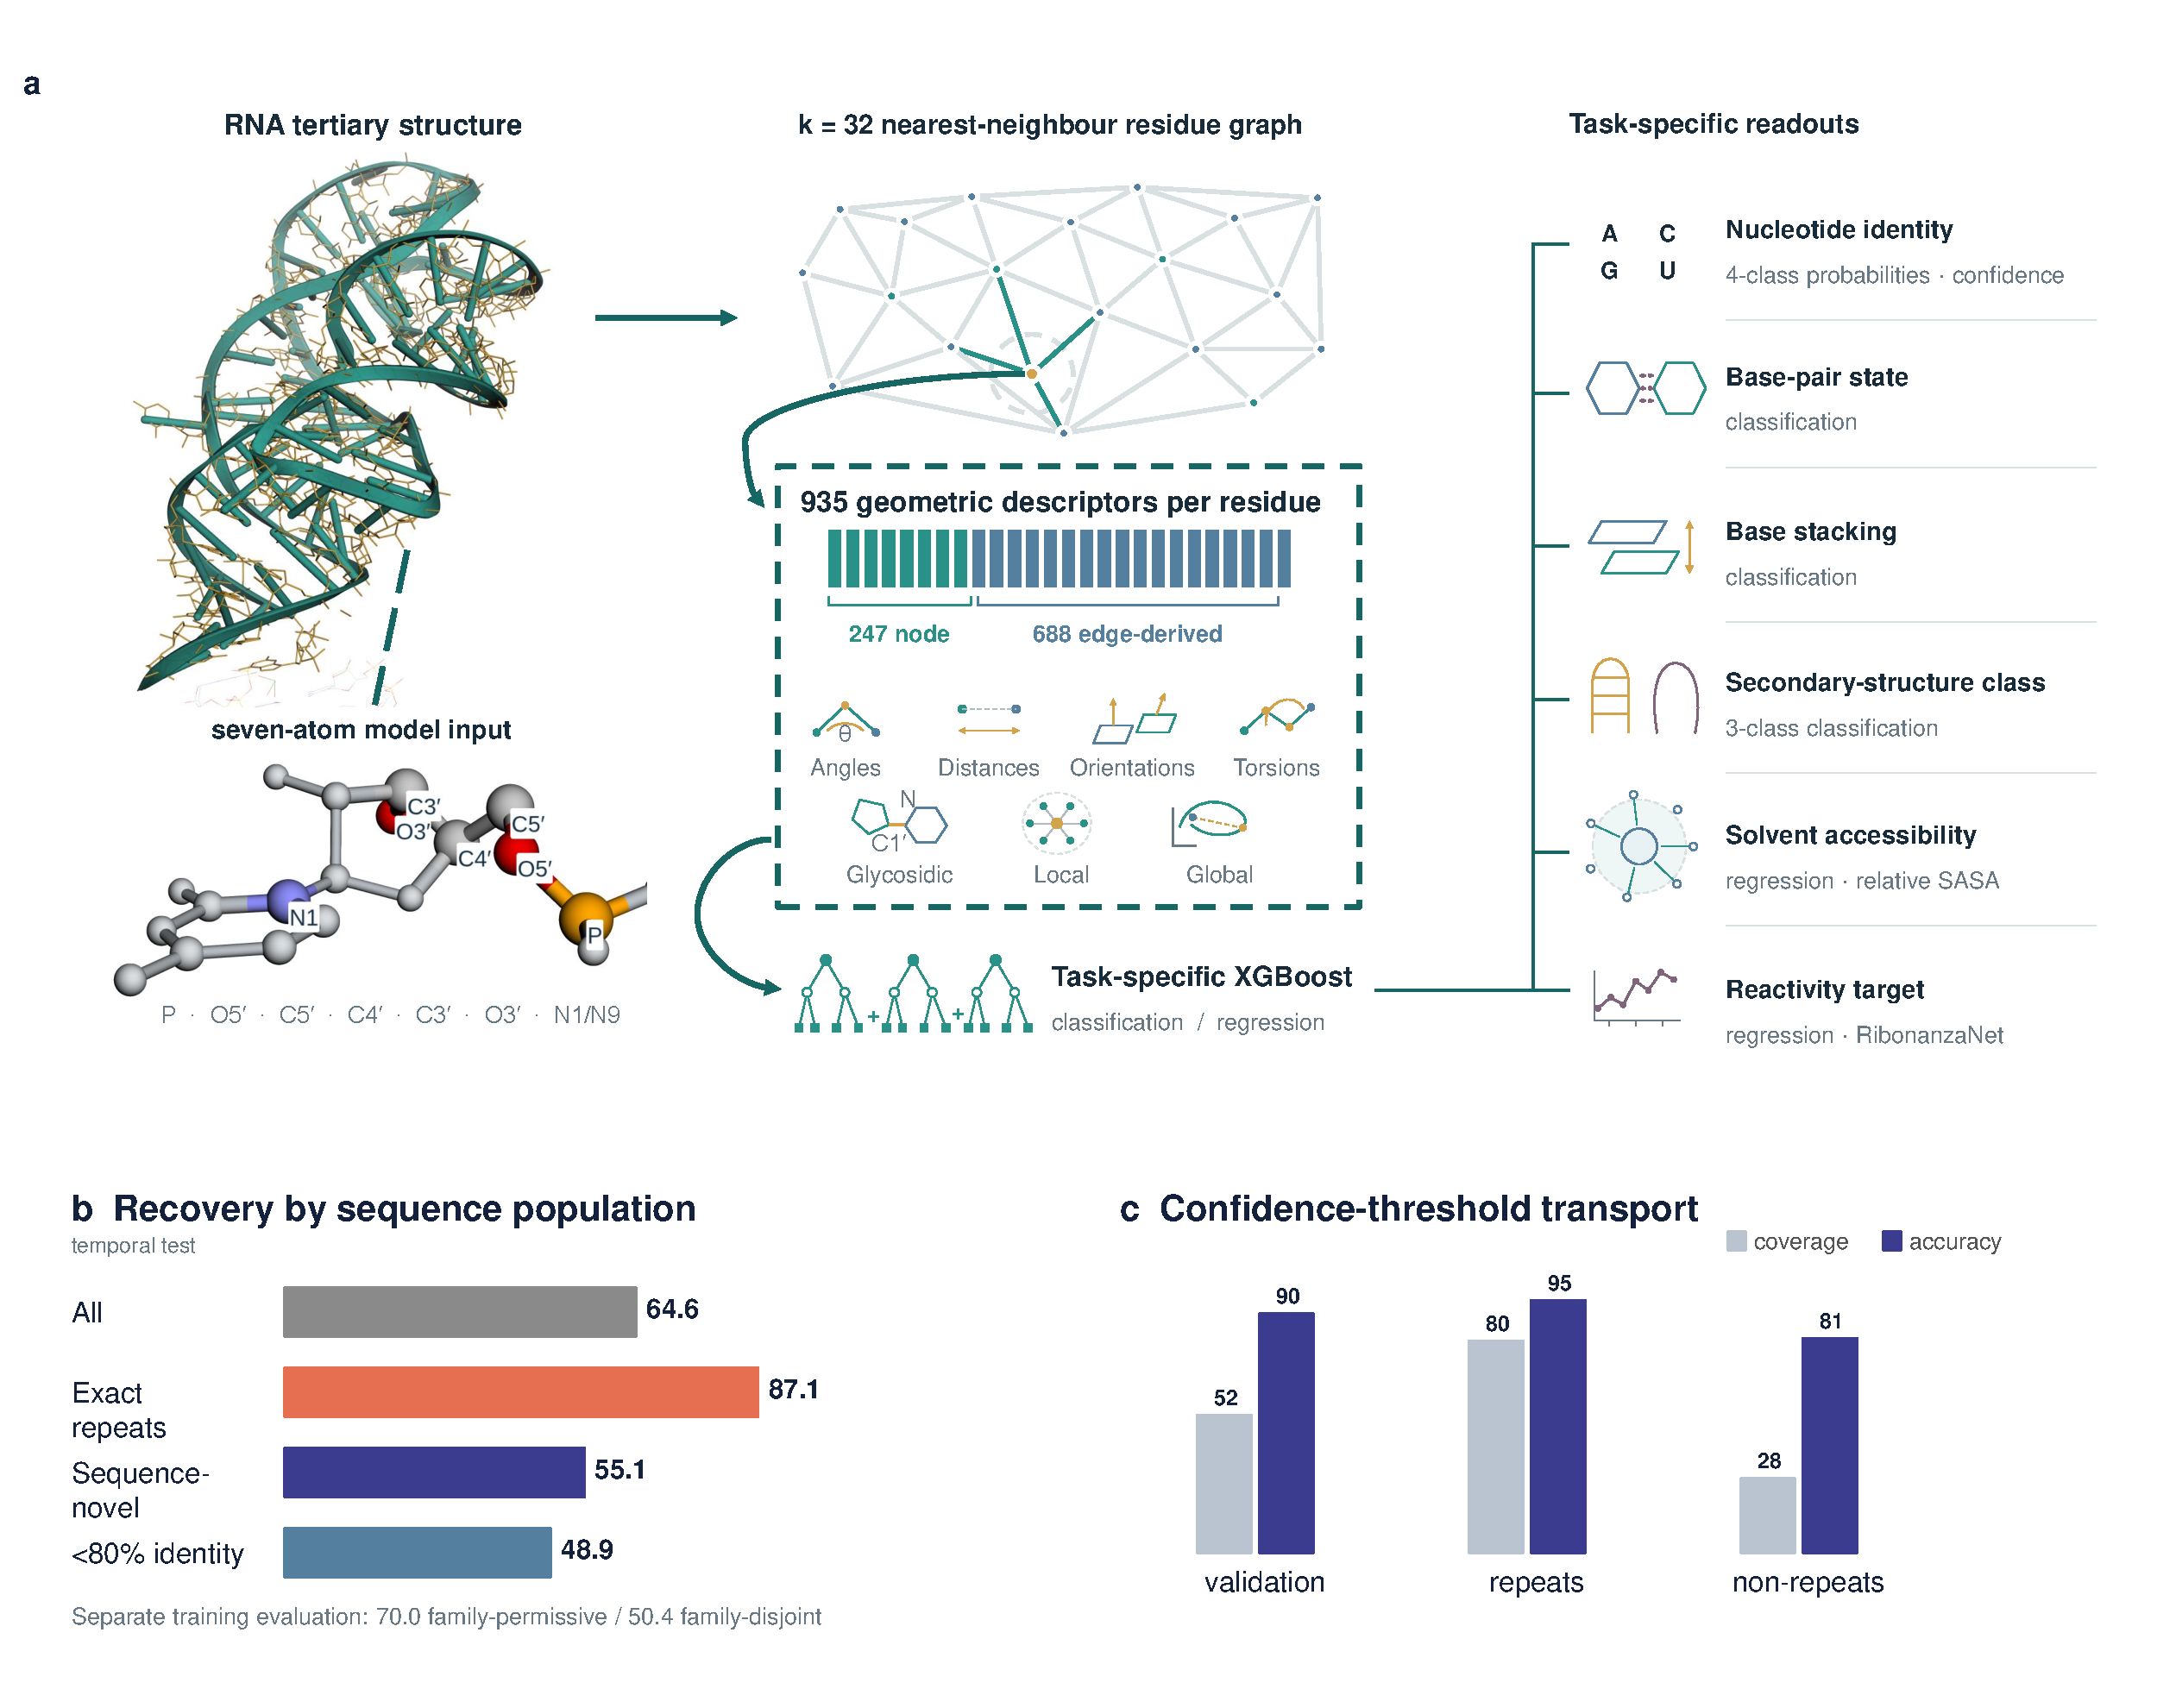
\includegraphics[width=\textwidth]{fig1_composite.pdf}
\caption{\textbf{A diagnostic framework for RNA backbone sequence recoverability.}
\textbf{a,} FORGE converts a seven-atom RNA backbone into 935 interpretable
geometric descriptors (247 node and 688 edge-derived features; $k=32$ residue
graph) and trains task-specific gradient-boosted models. The same representation
supports nucleotide identity and per-residue confidence, base pairing, stacking,
secondary-structure class, solvent exposure and a reactivity proxy. \textbf{b,}
Nucleotide recovery is not one quantity. In the temporal test, recovery is
64.6\% overall, 87.1\% on exact-sequence repeats, 55.1\% on sequence-novel chains
and 48.9\% below 80\% identity. A separate post-2025 training evaluation gives
70.0\% with family overlap and 50.4\% with entire families held out; these are not
nested temporal subsets. \textbf{c,} A fixed confidence threshold retains 51.9\%
of validation positions at 90.1\% accuracy, 79.9\% of repeats at 95.1\% and only
28.0\% of non-repeats at 80.8\%. Detailed uncertainty, task denominators and
design analyses are in Figs.~2--7 and the Supplementary Information.}
\label{fig:pipeline}
\end{figure}

\subsection{Temporal testing separates sequence-novel transfer from exact-sequence repeats}

We trained FORGE on 13,251 pre-2025 RNA chains and evaluated it on 4,135 post-2025
chains (291,331 unambiguous A/C/G/U positions). Overall weighted recovery reached 64.6\% (mean per-chain recovery, 63.4\%), but partitioning the temporal cohort by training overlap revealed a sharp divide: 1,281 evaluated chains (86,729 positions, 29.8\%) had an exact sequence match in the pre-2025 training set, whereas 2,854 chains (204,602 positions, 70.2\%) were sequence-novel. Recovery was 87.1\% on repeats and 55.1\% on novel chains; within Rfam families containing at least 20 chains
in both strata, repeats were 5.4--24.4 pp easier, and a chain-clustered model adjusting
for family and length gave +16.2 pp. Sequence-novel recovery is therefore our primary endpoint for transferable
nucleotide predictability. Maximum identity to any training sequence stratifies
recovery further: 85.0\% at $\ge$95\% identity, 67.4\% at 90--95\%, 62.8\% at 80--90\%
and 48.9\% below 80\% (Supplementary Table~S5). A cluster-disjoint temporal subset
(3,749 chains, 267,477 positions) gave 64.3\%, and the joint exact-novel
and cluster-disjoint subset (2,587 chains, 190,127 positions) gave 55.2\%.
The primary split is cluster-permissive (164 shared CD-HIT cluster IDs, 398 chains).
These values describe different restrictions and are not interchangeable:
55.1\% is the all-sequence-novel estimate, 55.2\% is the joint exact-novel,
cluster-disjoint subset, and 50.4\% comes from a separate post-2025 training evaluation with
entire families held out, not a further subset of the temporal cohort.

When evaluated on the exact FORGE position mask, public inverse-folding checkpoints reached 29.9\% (gRNAde), 32.9\% (RiboDiffusion) and 45.3\% (RDesign; Supplementary Table~S1). Because these public models retain their original training histories and were not retrained on the FORGE split, this comparison benchmarks off-the-shelf pretrained tools against an explicit geometric representation rather than isolating architecture differences.

Performance also varied sharply across RNA families and nucleotide classes: 5.8S rRNA (94.4\%), 5S rRNA (88.2\%) and tRNA (76.0\%) were easiest, whereas Purine (38.8\%) and K10\_TLS (29.5\%) were hardest (Fig.~\ref{fig:identifiability}c). Across bases, G showed the highest diagonal recovery (71.1\%) and U the lowest (57.8\%), being most often confused with C (Fig.~\ref{fig:identifiability}d).

\subsection{Recovery decomposes into memorisation, transfer and residual prediction error}
\label{sec:decomposition}

To compare family-permissive and family-disjoint transfer, we trained the same model architecture on post-2025 chains under two controlled splits. Under a sequence- and PDB-disjoint split that permitted Rfam families to cross between train and test (591 held-out chains, 53,288 positions), in-domain recovery reached 70.0\%, compared with 54.0\% for the frozen temporal model. Under a family-disjoint split (410 chains, 32,984 positions; zero shared sequences, PDBs or families), recovery was 50.4\% versus 47.5\% for the temporal model (50.2\% versus 46.9\% across the 365 sequence-novel chains, and 60.9\% versus 75.8\% on the 45 exact repeats). The 50.4\% family-disjoint estimate closely matches the 48.9\% observed below 80\% sequence identity in the temporal test; we therefore treat 70.0\% as a family-permissive upper reference and 50.4\% as a family-disjoint sensitivity estimate on the Rfam-labelled subset.

To test whether the confidence ordering is specific to gradient-boosted trees, we
trained a multinomial logistic model, an MLP and a $k$-nearest-neighbour classifier on
the same features and split. Absolute recovery was lower (39.2\%, 52.8\% and 46.3\%, respectively),
but recovery for all three rose monotonically with FORGE confidence; across the most confident 22\% of positions (confidence $\ge$0.9), they reached 64.3\%,
94.5\% and 91.5\% (FORGE 98.7\%), where the $k$NN estimate uses a 20,000-position query
subsample. The shared ranking identifies a common gradient of prediction difficulty,
while differences in absolute recovery retain a model-dependent contribution.
On unseen families, the remaining $\sim$50\% error combines Bayes ambiguity,
feature loss and model error. Distinguishing these contributions requires
additional representation and learner comparisons.

\begin{figure}[htbp]
\centering
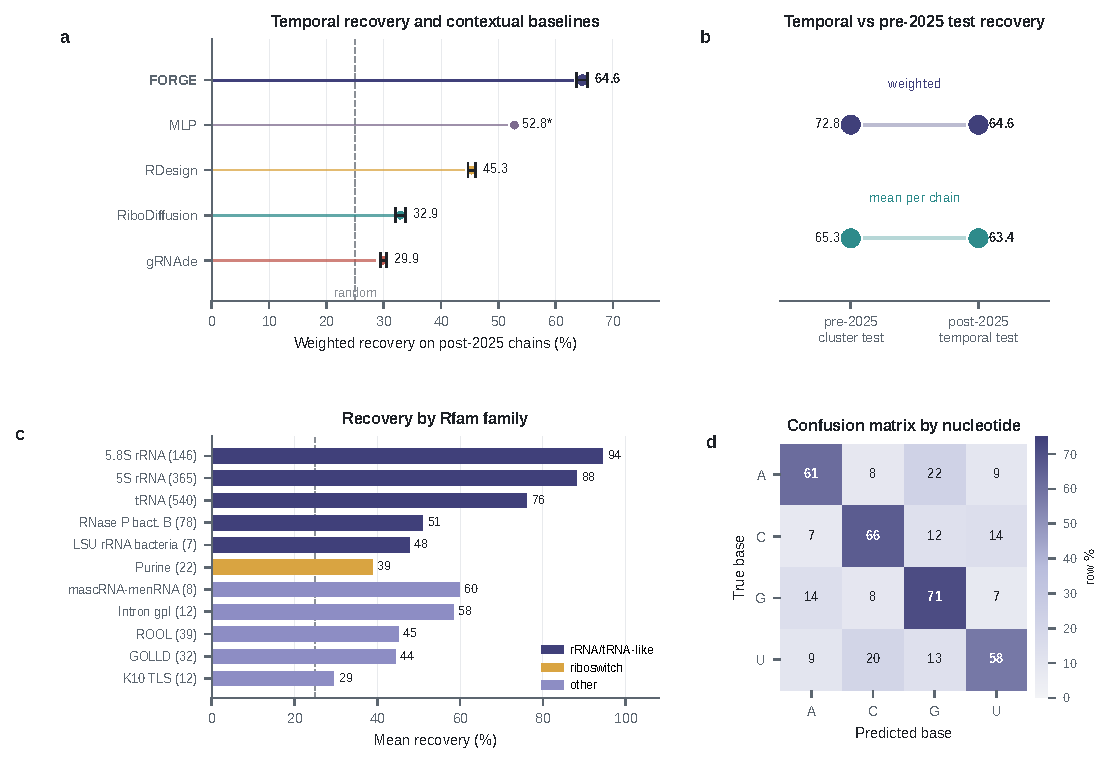
\includegraphics[width=\textwidth]{fig2_identifiability.pdf}
\caption{\textbf{Nucleotide identity is partially readable from backbone
geometry, but unevenly across families and bases.}
\textbf{a,} Weighted recovery of FORGE, a matched-budget MLP (52.8\%; the archived
59.5\% run is a different population) and public pretrained baselines on post-2025 RNA chains (horizontal lollipops;
black ticks, chain-bootstrap 95\% intervals where per-chain prediction
artifacts were available; the asterisk marks the MLP point estimate; dashed line, random recovery). Not a same-training benchmark; matched chains were 3,989 (gRNAde), 3,966
(RiboDiffusion) and 3,035 (RDesign; 3,966 evaluable); values are on the matched
mask (Supplementary Table~S1).
\textbf{b,} FORGE recovery on the pre-2025 cluster-held-out test and the
post-2025 temporal test, for length-weighted and mean per-chain recovery.
\textbf{c,} Mean per-family recovery for Rfam-labelled post-2025 chains,
coloured by broad RNA class, with chain counts in parentheses. \textbf{d,} Row-normalised confusion matrix
for the temporal per-position predictions; values are percentages within each
true nucleotide class.}
\label{fig:identifiability}
\end{figure}

\subsection{Sugar--phosphate geometry retains nucleotide-discriminating signal}
\label{sec:representation_controls}

To locate the geometric source of the nucleotide signal, we first summed the four-class probabilities into purine and pyrimidine calls, which classified chemical class at 82.2\% accuracy (mean per chain; random 50\%). Neutralising the N1/N9 coordinate before feature extraction and retraining on the full pre-2025 set still retained 58.5\% recovery across the 4,135 chains and 291,331 positions—6.1 pp below the seven-atom model—alongside 72.2\% purine/pyrimidine accuracy.

Because zeroing a coordinate does not remove atom-dependent features, we also trained matched-budget
seven-atom, N-neutralised, five-atom and three-atom models after masking every feature
whose definition depends on the target atom (Methods; Supplementary Table~S4). The seven-atom control reached a matched baseline of
61.94\%, the N-feature-removed model 58.50\% (3.43 pp lower), and the
origin-zeroed and C4$'$-dummy-anchor models 57.25\% and 57.42\%; the dummy anchor differs
from zeroing by only $+0.17$ pp, so the artificial origin is not a material
confound. Masking 257 O5$'$/O3$'$- and 435 O5$'$/C5$'$/C3$'$/O3$'$-dependent features
cost 0.31 and 0.90 pp, indicating strong redundancy among sugar descriptors; these are
lower bounds (Supplementary Table~S4). A rigid-rotation audit gave 59.0\% prediction agreement
(41.0\% changed) and reduced recovery from 59.3\% to 47.9\%; a rotation-masked model
retained 62.1\% unrotated recovery but only 53.3\% agreement under transformation. A canonicalised-frame
model recovered 62.3\% with 99.6\% agreement and reproduced the decomposition
(84.7/52.8/47.0\%; ECE 0.012) at a cost of 2.35~pp
(Supplementary Table~S7).

Non-parametric analyses of the 935-dimensional feature space reinforced this view under a leave-one-chain-out design: a $k=10$ nearest-neighbour classifier matched XGBoost almost exactly (53.6\% versus 53.9\%), with accuracy dropping from 81.5\% to 44.9\% as local label entropy increased (Spearman $\rho=+0.227$; Supplementary Fig.~S7a). A feature ontology covering 889 of 935
dimensions showed that U/C discrimination concentrates in base-orientation and stacking
features, whereas A/G discrimination is weaker and more distributed
(Supplementary Fig.~S7b).

\begin{figure}[htbp]
\centering
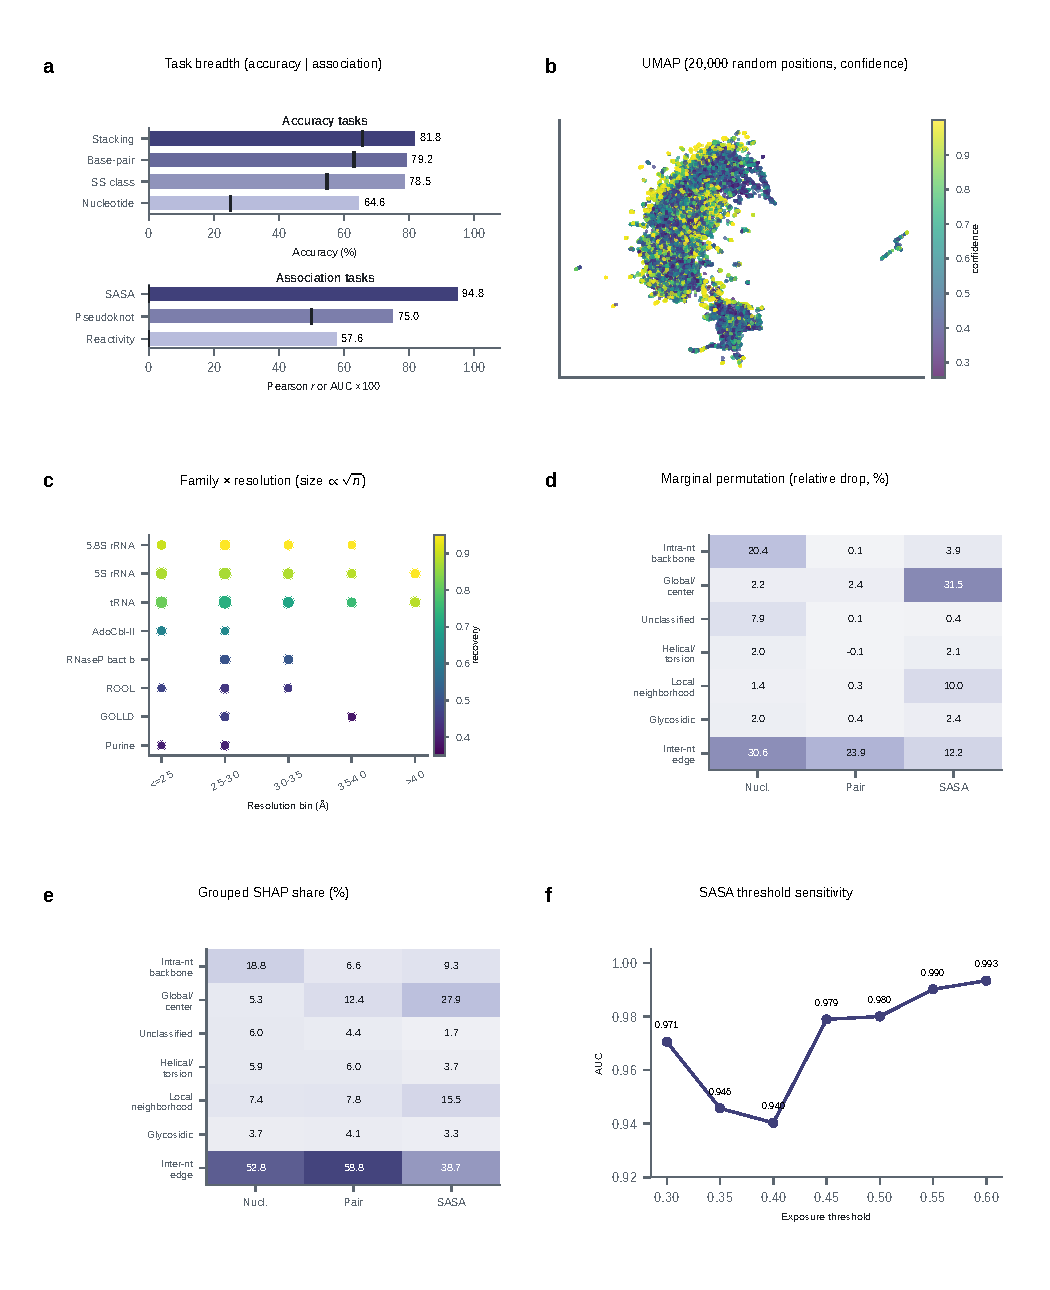
\includegraphics[width=\textwidth]{fig3_information_landscape.pdf}
\caption{\textbf{Information landscape across readouts, feature space and strata.}
\textbf{a,} Task breadth split into accuracy tasks (nucleotide, base-pair, stacking,
three-class secondary structure) and association tasks (SASA Pearson $r$, pseudoknot
AUC, reactivity $r$); marker, chance or majority baseline. Denominators are 291,331 positions for nucleotide/SASA, 182,338 for base-pair,
290,878 for stacking, 163,395 for SS class and 299,074 for reactivity.
\textbf{b,} UMAP of 20,000 random post-2025 positions with finite confidence, coloured
by confidence. \textbf{c,} Family $\times$ resolution recovery; bubble size $\propto\sqrt{\text{chains}}$; colour, weighted recovery. \textbf{d,}
Marginal permutation importance (relative metric drop) for nucleotide, base-pair and
SASA. \textbf{e,} Grouped SHAP share for the same readouts (conditional on the model).
\textbf{f,} SASA AUC as a function of the exposure threshold. Source data are indexed in
the Supplementary Information.}
\label{fig:controls}
\end{figure}

\subsection{Descriptor groups and retrospective strata}
\label{sec:feature_strata}

Marginal permutation of the frozen models measures reliance rather than necessity (Fig.~\ref{fig:controls}d): nucleotide identity relied most on inter-nucleotide edge
(30.6\% relative drop) and intra-nucleotide backbone (20.4\%) geometry; base-pair state on edge geometry (23.9\%);
and solvent accessibility on global/centre (31.5\%) and local-neighbourhood
(10.0\%) descriptors. Grouped SHAP agreed on edge dominance but gave SASA more edge weight, reflecting correlated groups. Leave-one-group-out retraining cost 1.7--2.2~pp of nucleotide recovery when edge
or intra-nucleotide backbone features were removed, whereas removing any single group changed SASA $r$ by less than
1~pp; these rankings are descriptive (Supplementary Table~S10). Zeroing explicit SASA, global/centre and density features lowered $r$ from
0.948 to 0.942, supporting packing-associated predictability, not independent chemistry (Supplementary Fig.~S12b). 

RNA family dominated recovery variation: relative to the pooled remainder,
5.8S rRNA gained $+33.9$~pp, 5S rRNA $+24.9$~pp and tRNA $+18.6$~pp (BH
$q<10^{-60}$), whereas RNase P did not differ significantly ($+1.0$~pp; $q=0.50$). Resolution had no
clear linear association ($+1.1$~pp per \AA{}; $p=0.10$).
Several nonlinear or subgroup terms were significant after BH correction within their
declared families: a spline test ($q=0.0014$), the $>4.0$~\AA{} bin ($+5.4$~pp;
$q=0.0035$), a family interaction ($q=0.028$) and the X-ray-only coefficient
($+4.5$~pp per \AA{}; $q=0.028$). The X-ray-versus-cryo-EM method term was $+1.8$~pp
($p=0.26$), and the within-X-ray resolution slope was $+4.5$~pp per \AA{}
($q=0.028$); these are distinct estimands. Length contrasts were not significant
(all $q>0.7$). We interpret resolution and length as composition-confounded,
not quality effects (Supplementary Tables~S9 and S10).

\subsection{The same representation supports stacking and secondary-structure class}

The same descriptors predicted base-plane stacking at 81.8\% accuracy (AUC 0.879
without explicit stacking features) and three-class secondary structure at 78.5\% accuracy (macro $F_1=0.542$;
pseudoknot AUC 0.750 but $F_1<0.001$ at the argmax threshold). The stacking label is
heuristic: distance and angle variations alter fewer than 0.5\% of labels, whereas a $\pm0.5$~\AA{}
vertical offset alters 22--61\%, making this readout exploratory. UMAP placed high-confidence positions in distinct regions of the representation
(Fig.~\ref{fig:controls}a,b). 

\subsection{Context analyses specify the interpretation of nucleotide confidence}

Ligand-specific positions were more confidently recovered than non-binding positions
(0.755 versus 0.702; 42 contacts), but the PDB-clustered difference was uncertain
($+0.053$; Fig.~\ref{fig:context}a,b). The contrast is an association from coordinate-only predictions: the model
does not see ligands, and the in-range joins are not residue-ID-validated contacts. Across nine post-2025 NMR ensembles, mean P-atom
displacement was not consistently related to confidence (mean $\rho=0.16$; two of nine
negative; Fig.~\ref{fig:context}c), so confidence is not a validated flexibility or
dynamics measure. A two-ensemble per-conformer pilot (1A60/1BYJ, 70 positions) gave a
call-switch rate of 0.255, with higher switching in the high-feature-variation tertile
(0.272 versus 0.175); this is a bounded pre-2025 sensitivity analysis, not a general
ensemble result. Continuous base-plane stacking geometry was also only weakly related to
confidence (200 chains, 13,801 unique positions; pooled $\rho=0.008$; mean within-chain
$\rho=0.060$; controlled coefficient $+0.041$, cluster
$p=2.9\times10^{-13}$), so confidence is not a simple stacking-order proxy.

\subsection{Confidence identifies high-accuracy subsets and chain-level failure modes}

Confidence scores isolate a high-accuracy regime within the temporal test. On the full 4,135-chain
temporal set (291,331 positions), FORGE had an expected calibration error of 0.023 and a pooled accuracy of 64.6\% (Fig.~\ref{fig:calibration}a).
Removing the least-confident 50\% of positions raised retained accuracy to 85.1\%, and
removing 75\% to 97.8\% (Fig.~\ref{fig:calibration}b). Errors concentrate at low confidence (Fig.~\ref{fig:calibration}c); calibration was 0.011 on
sequence-novel chains and 0.051 on repeats. A confidence threshold (0.61) selected on a 1,000-chain pre-2025
validation subset for 90\% selective accuracy retained 52\% of validation positions at
90.1\% accuracy, but retained 44\% of post-2025 positions at 88.7\% accuracy; coverage was 80\% (95.1\% accurate) on
repeats and 28\% (80.8\%) on non-repeats, showing that threshold transport depends on sequence novelty (Supplementary Table~S15).

At the chain level, reaching 90\% retained-position accuracy required abstaining from a median of 85\% of residues across the post-2025 cohort: 26\% of chains needed fewer than 30\% of positions removed, whereas 41\% failed to reach the 90\% target even after 90\% removal (evaluated on chains with at least 5 positions using a 10\% removal grid; Fig.~\ref{fig:calibration}d). The audit therefore reports both high-confidence annotation opportunities and chain-level failure modes.

\begin{figure}[htbp]
\centering
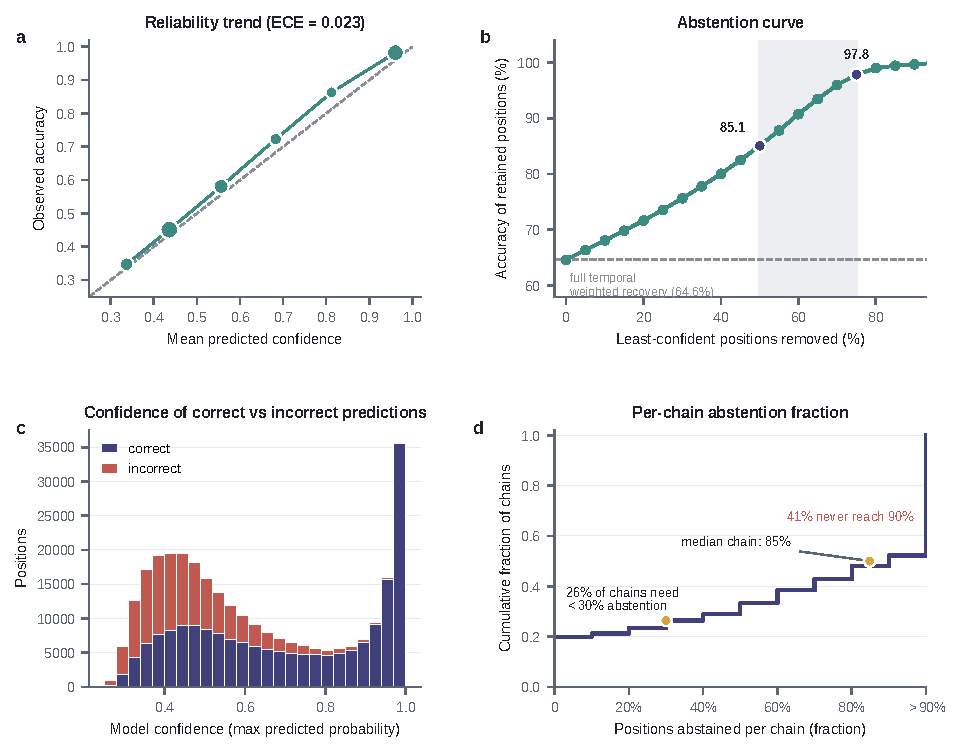
\includegraphics[width=\textwidth]{fig4_calibration.pdf}
\caption{\textbf{Confidence calibration and abstention.} \textbf{a,}
Reliability trend from retained post-2025 predictions (marker size, positions
per bin; ECE, full temporal set).
\textbf{b,} Pooled abstention curve on the full temporal set; the dashed line marks
full temporal weighted recovery. \textbf{c,} Stacked histogram of model confidence
for correct and incorrect per-position predictions on the full temporal set.
\textbf{d,} Per-chain abstention fraction required to reach 90\% retained accuracy;
chains in the $>$90\% bin did not reach the target.}
\label{fig:calibration}
\end{figure}

\subsection{A shared representation maps task-specific structural readouts}

To map structural predictability across properties, we trained separate XGBoost models on the shared 935-dimensional representation
for three additional labels spanning direct geometry, local packing and partial
backbone exposure: DSSR
base-pair state~\citep{lu2015dssr}, relative solvent accessibility and a
RibonanzaNet-derived reactivity target.

 Nucleotide identity
showed the strongest four-class signal (64.6\% weighted recovery; random 25\%).
Base-pair state, tightly coupled to A-form geometry, was predicted at 79.2\% accuracy
against a 63.1\% majority baseline (AUC 0.880). The RibonanzaNet-derived reactivity
target was captured at intermediate strength (Pearson $r=0.576$, $R^2=0.329$),
consistent with reactivity depending on both local conformation and nucleotide
chemistry in probing assays~\citep{zubradt2017dms}. Each readout retains its own label definition, metric and baseline.

Relative solvent accessibility—a full-atom label rather than an input—was also strongly
predictable on the same cluster-permissive temporal split: Pearson $r=0.948$, $R^2=0.899$ and binary AUC 0.936 (training-median threshold 0.395; 44.9\% exposed). This readout captures coordinate-derived packing and accessibility.

Crucially, FORGE nucleotide confidence was only weakly associated with these auxiliary properties: it did not predict base-pair state (AUC 0.49) and correlated only weakly with solvent accessibility ($r=-0.08$) and the reactivity target ($r=0.03$). Nucleotide confidence therefore reflects the certainty of the base call itself rather than acting as a generic proxy for pairing or burial.

\begin{table}[htbp]
\caption{\textbf{Task-specific readouts from the same backbone descriptors.}
All tasks use the same 935 geometric descriptors computed from RNA coordinates;
task labels are used only as supervision and are not input features. Solvent exposure and
stacking labels are computed from full-atom coordinates, not from the seven-atom input. DMS
denotes a RibonanzaNet-derived reactivity target rather than measured chemical
probing. Evaluation-set sizes and split definitions are reported in
Supplementary Tables~S1 and S3. Nucleotide identity is reported for all chains (64.6\%), exact-sequence-novel chains (55.1\%) and chains below 80\% identity (48.9\%); the all-chain value is inflated by exact-sequence repeats.}
\label{tab:readouts}
\centering
\begingroup
\footnotesize
\setlength{\tabcolsep}{3pt}
\renewcommand{\arraystretch}{1.18}
\begin{tabular}{@{}L{0.13\textwidth}L{0.17\textwidth}L{0.18\textwidth}L{0.13\textwidth}L{0.31\textwidth}@{}}
\toprule
Task & Label source & Primary metric and reference & Result & Interpretation and controls \\
\midrule
Nucleotide identity & PDB sequence & Weighted recovery; random 25\% & 64.6\% overall; 55.1\% sequence-novel & Primary output; the gap between 87.1\% on exact repeats and 55.1\% on novel chains quantifies repeat inflation \\
Base-pair state & DSSR paired/unpaired label & Accuracy and AUC; majority 63.1\% & 79.2\%; AUC 0.880 & Confidence association AUC $-$ 0.5 = $-$0.01; no DSSR, dot-bracket or pair labels used as features \\
Solvent exposure & Full-atom relative SASA & Pearson r and R$^2$; binary AUC & r=0.948; R$^2$=0.899; AUC 0.936 & Confidence association $r=-0.08$; local-packing signal; full-atom label, seven-atom input \\
Reactivity target & RibonanzaNet-inferred & Pearson $r$ and $R^2$; null $r=0$ & $r=0.576$; $R^2=0.329$ & Confidence association $r=+0.03$; intermediate accessibility/chemistry-associated layer, not a measured DMS predictor \\
Stacking & Full-atom base-plane label & Accuracy and AUC; chance from label balance & 81.8\%; AUC 0.879 without explicit stacking descriptors & Heuristic label; offset-threshold sensitive; exploratory \\
Secondary-structure class & DSSR 3-class label & Accuracy, macro $F_1$, pseudoknot AUC & 78.5\%; $F_1=0.542$; AUC 0.750 & Pseudoknot $F_1<0.001$ at argmax; AUC 0.750; descriptive class labels \\
\bottomrule
\end{tabular}
\endgroup
\end{table}

\subsection{Pre-specified case studies illustrate where the audit is usable}
\label{sec:cases}

To illustrate how these residue-level outputs behave on individual structures, we applied four pre-specified selection rules (Methods) and report all resulting audit cards (Fig.~\ref{fig:cases}). Recovery spanned 100\% on the confidence-selected positive control, 34.8\% on the family-targeted Purine riboswitch, 50\% on the outcome-blind pseudoknot and 37\% on the outcome-blind median-length novel chain, making the residue-level audit explicit across both confident and difficult folds.

\subsection{Compatibility, foldability and design score are separable}

Beyond single-position calls, FORGE cross-entropy (CE) scores full-chain sequence--backbone compatibility. Across 50 post-2025 chains, native sequences ranked above composition-preserving and secondary-structure-context shuffles with near-perfect AUC (0.99--1.00), above gRNAde and RiboDiffusion designs (AUC 0.98) and above compensatory pair-swap mutants (AUC 0.89; Supplementary Fig.~S6a). RDesign was the sole exception (native-above-decoy AUC 0.41), frequently assigning lower CE to its designs than to native sequences. 


Among 8,125 pseudoknot designs, FORGE CE was positively associated with the
experimental SHAPE-based score, but more weakly than RNAfold MFE F1. In the 1,656-design complete-case subset, the partial Spearman correlation was $+0.549$ after controlling for MFE F1 and $+0.123$ after also controlling for GC content and length; FORGE CE contributed $\Delta R^2=0.022$ ($p=4.3\times10^{-12}$; Supplementary Fig.~S6b,c). This complete-case association is exploratory and has not been cluster-corrected. Pooled Spearman $\rho$ was 0.289, whereas normalised within-puzzle rank correlation was 0.078
and held-out-target $\rho$ was 0.088. Adding CE to an MFE+GC+length baseline yielded only a small
held-out improvement ($\rho=0.332$ versus 0.316; $\Delta=+0.016$; 13/21 puzzles positive), providing
no evidence of a transferable success ranker (Fig.~\ref{fig:design}a,b and Supplementary Table~S13).
This gap between near-perfect decoy discrimination and modest target-held-out experimental ranking demonstrates that sequence--backbone compatibility, foldability and empirical design performance represent distinct evaluation axes.

\subsection{Solved AI-designed pseudoknots distinguish successful generation from read-back}

To test whether the diagnostic signal generalises to non-natural backbones, we
applied the frozen model to cryo-EM structures from the OpenKnot AI
pseudoknot-design study~\citep{townley2026openknot}: PDB entries 10ZT
(gRNAde), 10ZU (MPNN-fixbb), 11EH (Struct2Seq) and 11AG (MPNN-RFdiff, two
chains), downloaded on 2026-05-24 and processed with the locked checkpoint.
Best training-set sequence identities were 34--39\%, below the prespecified
threshold (Supplementary Table~S2). FORGE retained above-random recovery on
all five chains (54.2\%, 41.7\%, 36.5\%, 43.6\% and 44.6\%;
Supplementary Fig.~S6d), while public pretrained baselines were at or
below random (gRNAde 7--15\%, RiboDiffusion 13--25\%, RDesign 11--40\%). Strikingly, on the gRNAde-designed structure 10ZT, gRNAde itself recovered just 12.5\% of its own design sequence in standard inference mode, whereas FORGE recovered 54.2\% from the same experimental coordinates—demonstrating that a generative model can produce a successful fold without providing an invertible readout of backbone geometry.

Mean per-position
confidence was 0.43--0.46 on these structures (versus 0.48 on the full
post-2025 set), only 1--7\% of positions exceeded the 0.7 high-confidence
threshold, and 11 of those 19 high-confidence calls (57.9\%) were correct
(Supplementary Fig.~S4a,b). Confidence was lower out-of-distribution, but this sample is
too small for a calibrated OOD guarantee. The
N-free control was heterogeneous across design strategies: recovery on 10ZT
dropped by 16.7 percentage points (54.2\% to 37.5\%) and on 11AG by 10--12
points, whereas 10ZU and 11EH were essentially unaffected, suggesting that
different design methods encode the glycosidic-anchor position differently.
Purine/pyrimidine accuracy remained above chance on all chains (7-atom,
65--72\%; N-free, 50--62\%; random 50\%; Supplementary Fig.~S4c).

A forward-folding control tested the reverse direction. We submitted the scaffold-embedded constructs to
AlphaFold~3~\citep{abramson2024alphafold3} with three sequence classes per
construct: the true design sequence, the FORGE-derived sequence and the
FORGE-derived sequence after R-Net-guided reactivity refinement (Methods).
Only the true 10ZT sequence returned a near-experimental fold (6.6~\AA{}
P-RMSD; all 38 native Watson--Crick pairs recovered). The remaining true
sequences did not reproduce the experimental fold (14--27~\AA{} P-RMSD) despite
mostly correct base pairing (SS $F_1$ 0.69--0.88), and none of the evaluated FORGE-derived or RNet-refined AF3 models (four constructs,
including scaffolded and free/dimer variants) produced an AF3-consistent fold
(SS $F_1 \le 0.36$; Supplementary Figs.~S1 and S2). That AlphaFold~3 did not reproduce the experimental fold for three of the four experimentally solved controls underscores that forward-folding agreement does not substitute for experimental validation. In this cohort, FORGE-derived read-back sequences did not yield AF3-consistent structures, leaving physical foldability an independent experimental question (Fig.~\ref{fig:design}c). At the 11AG dimer interface, accuracy was 30.0\%/35.0\%
versus 52.5\%/50.8\% outside the interface despite similar confidence, separating
interface errors from intrachain errors (Fig.~\ref{fig:design}d).

\begin{figure}[!p]
\centering
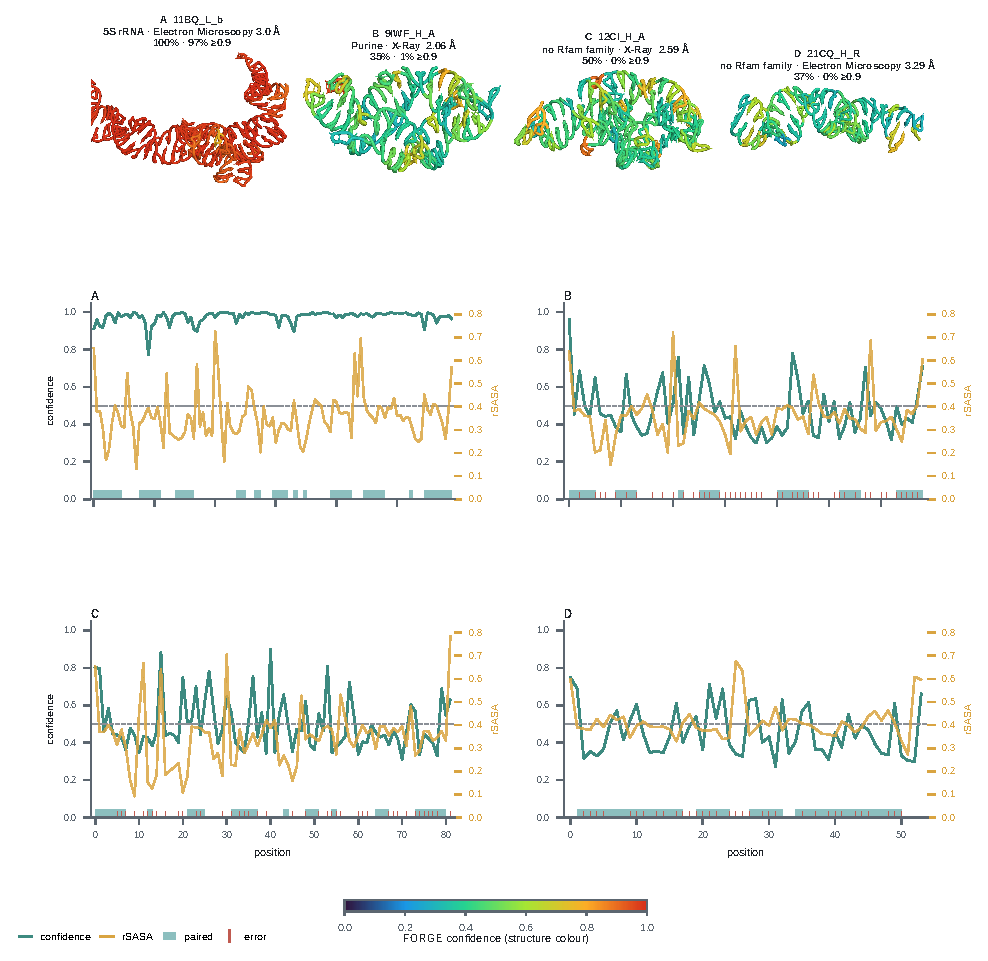
\includegraphics[width=\textwidth]{fig5_case_studies.pdf}
\caption{\textbf{Pre-specified per-position audit cards.}
Four chains selected by rules frozen before outcome inspection: \textbf{A},
high-resolution/high-confidence 5S rRNA (11BQ\_L\_b); \textbf{B}, Purine riboswitch
(9IWF\_H\_A); \textbf{C}, pseudoknot chain with at least 10 DSSR pseudoknot positions
(12CI\_H\_A); \textbf{D}, median-length exact-novel, cluster-disjoint chain
(21CQ\_H\_R). PyMOL cartoon of the RNA backbone coloured by FORGE confidence (rainbow, 0--1;
low, dark blue; high, red); thin sticks, base atoms. Bottom, merged per-position tracks:
confidence (teal, left axis), rSASA (orange, right axis) and paired positions (blue
bars); red ticks mark errors. Titles give family, method, resolution, recovery and the
fraction of positions with confidence $\geq0.9$. Descriptive cards.}
\label{fig:cases}
\end{figure}

\begin{figure}[!p]
\centering
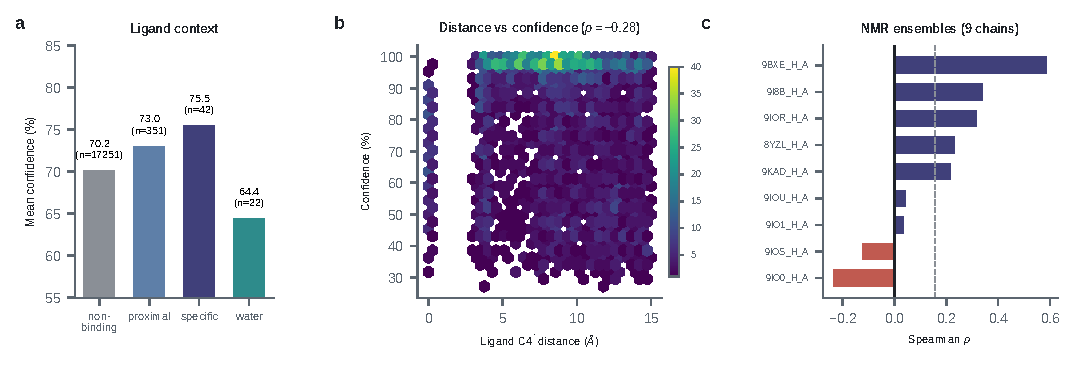
\includegraphics[width=\textwidth]{fig6_context.pdf}
\caption{\textbf{Context and ensemble boundaries.}
\textbf{a,} Mean confidence for non-binding, ligand-proximal, ligand-specific and
water-proximal positions in 200 post-2025 ligand-annotated chains. \textbf{b,} Minimum
ligand C4$'$ distance versus confidence (Spearman $\rho=-0.28$); the specific-versus-
non-binding difference has a PDB-clustered interval crossing zero. \textbf{c,} Per-chain
Spearman correlation between NMR ensemble mean P-atom displacement and confidence for
nine post-2025 ensembles (mean $\rho=0.16$; dashed). Ligand and NMR analyses are
descriptive; absence of a modelled ligand is not evidence of non-binding.}
\label{fig:context}
\end{figure}

\begin{figure}[!p]
\centering
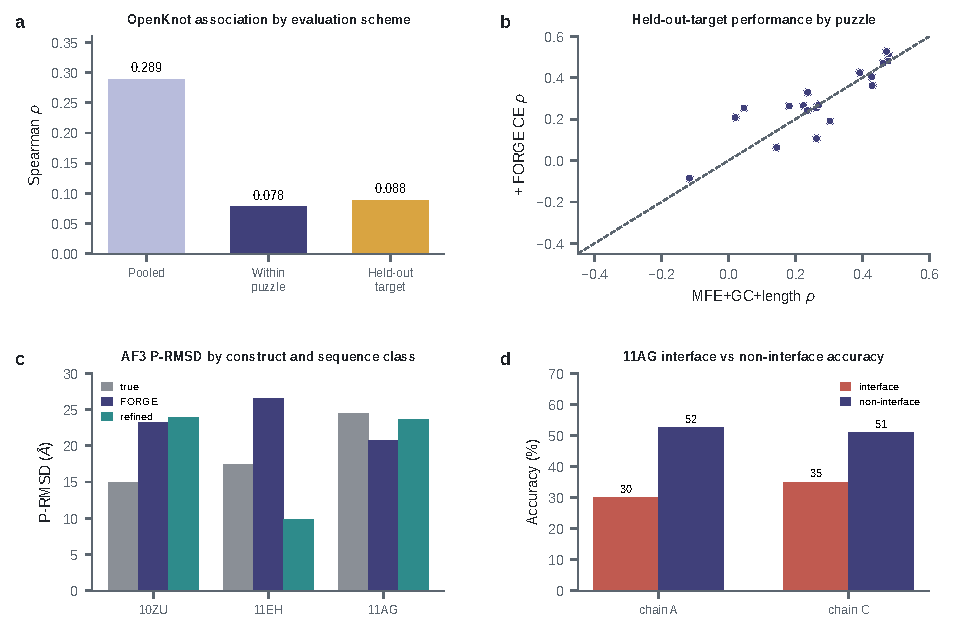
\includegraphics[width=\textwidth]{fig7_design_audit.pdf}
\caption{\textbf{Design-score and interface audit.}
\textbf{a,} OpenKnot association under pooled, normalised within-puzzle and
target-held-out evaluation. \textbf{b,} Per-puzzle held-out-target Spearman for an
MFE+GC+length baseline versus the same model plus FORGE CE; the mean increment is small
and mixed across puzzles. \textbf{c,} AF3 P-RMSD for true, FORGE-derived and
RNet-refined sequences of three constructs; 10ZT is omitted from this panel because
its derived/refined models were reported separately; the Results text summarizes
all evaluated generated and refined variants. \textbf{d,} 11AG interface versus
non-interface accuracy for the two chains; confidence was similar, so interface errors
are not a confidence effect.}
\label{fig:design}
\end{figure}

\clearpage
